\chapter{Предобработка данных}

Машинное обучение является мощным и эффективным инструментом при реализации
алгоритмов классификации, маршрутизации, обработки и поиска документов, однако, определяющее значение в этих процессах имеет качество исходных данных \cite{bib2}. Именно поэтому проведение подготовки исходных документов, их предварительная обработка позволяет значительно повысить точность результатов, получаемых в ходе применения
машинного обучения. Разобьем этот этап на 6 шагов.

\begin{enumerate}

\item На вход поступает множество документов определенных форматов (txt, doc или pdf, как в нашем случае). Выбирается библиотека программного кода в зависимости от формата исходного документа и осуществляется извлечение данных из документа в виде неформатированного текста. Этот шаг уже произведен платформой \textit{Kaggle}. Общее количество электронных писем --- 7945.

\item В текстовом файле, взятом из \textit{Kaggle}, могут быть пропущенные данные (например, в связи с плохим качеством pdf-файла). Такие данные пропускаются и нами не обрабатываются. После осуществления этого шага остается 6742 писем. 

\item Текст каждого электронного письма проходит процесс нормализации --- удаляются знаки препинания, выделяются отдельные слова. После этого каждое слово приводится в нижний регистр. 

На этом шаге для дальнейшего анализа можно посмотреть на различного рода статистики.
Ниже приведена гистограмма распределения количества слов каждой длины: 

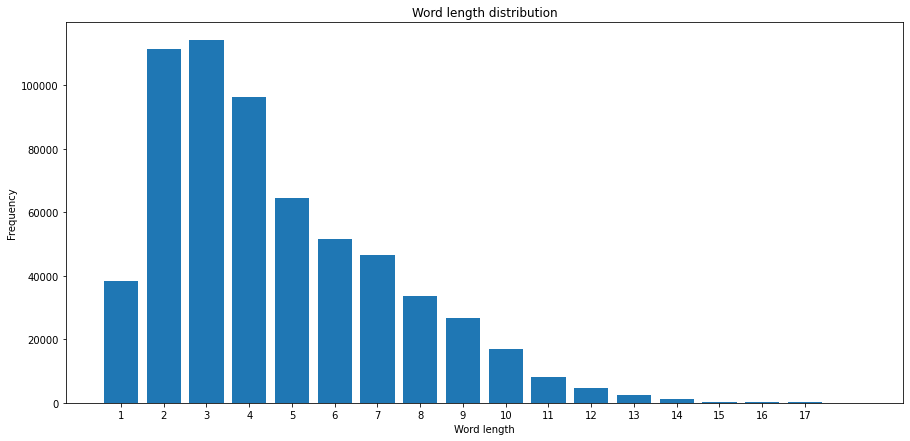
\includegraphics[scale=0.5]{pics/word_lengths.png}

А ниже приведена гистограмма распределения количества электронных писем каждой длины: 

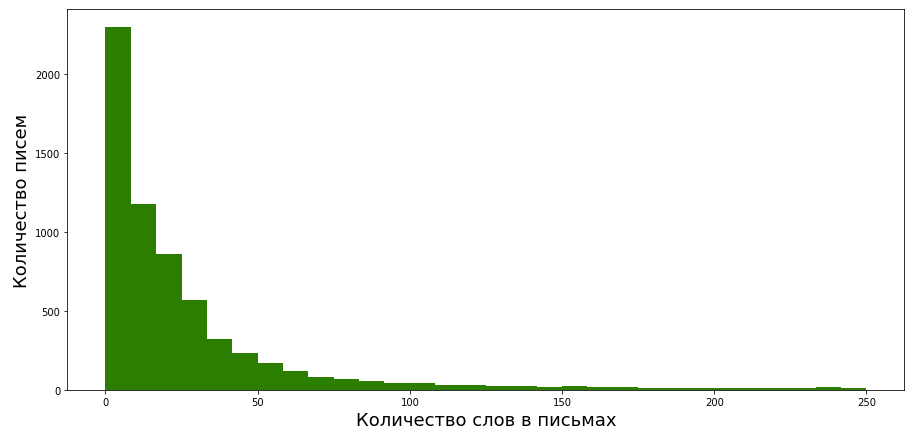
\includegraphics[scale=0.5]{pics/email_lengths.png}

\item Дальше происходит фильтрация текста по стоп-листу --- набору коротких слов (артиклей, предлогов, местоимений), не несущих большой смысловой нагрузки, что приводит к сокращению объема текста и повышению его смысловой ценности. 

\item Следующим шагом происходит лемматизация --- процесс приведения слов к леммам, т. е. нормальным словесным формам. Для реализации лемматизации можно использовать библиотеку программного кода \textit{spaCy} \cite{bib3}, позволяющую привести все слова к нормальной форме. Полученный после выполнения лемматизации набор слов уже может использоваться для проведения машинного обучения и решения конкретных задач. 

\item Индексация --- построение некоторой числовой модели текста, которая переводит текст в удобное для дальнейшей обработки представление. 
 
\end{enumerate}


% \section{Тематическое моделирование}

Тематическая модель (англ. \textit{topic model}) — модель коллекции текстовых документов, которая определяет, к каким темам относится каждый документ коллекции. Алгоритм построения тематической модели получает на входе коллекцию текстовых документов. На выходе для каждого документа выдаётся числовой вектор, составленный из оценок степени принадлежности данного документа каждой из тем. Размерность этого вектора, равная числу тем, может либо задаваться на входе, либо определяться моделью автоматически.

Тематическое моделирование (англ. \textit{topic modeling}) — построение тематической модели.

Задача построения тематической модели звучит следующим образом. Задана коллекция текстовых документов $D$. Каждый документ $d$ из коллекции $D$ представляет собой последовательность слов $W_d=(w_1,\ldots,w_{n_d})$ из словаря $W$, где $n_d$ — длина документа $d$. Предполагается, что каждый документ может относиться к одной или нескольким темам. Темы отличаются друг от друга различной частотой употребления слов. Требуется найти эти темы, то есть определить
\begin{itemize}
\item число тем;
\item распределения частот слов, характерное для каждой темы;
\item тематику каждого документа — в какой степени он относится к каждой из тем.
\end{itemize}

Данная задача может рассматриваться как задача одновременной кластеризации документов и слов по одному и тому же множеству кластеров, называемых темами. Строится, так называемая, мягкая кластеризация, то есть один документ может принадлежать нескольким темам в различной степени.

Для тематического моделирования в качестве модели в данной работе используется латентное размещение Дирихле (англ. \textit{latent Dirichlet allocation, LDA}) \cite{bib4}.

Для оценки качества данной модели используется перплексия (англ. \textit{perplexity}) --- оценка того, насколько хорошо вероятностная модель предсказывает выборку. Низкая перплексия указывает на то, что распределение вероятностей хорошо предсказывает выборку. 

В зависимости от параметра модели, отвечающего за количество тем у распределения текстов, получилась следующая зависимость значения перплексии от количества тем:

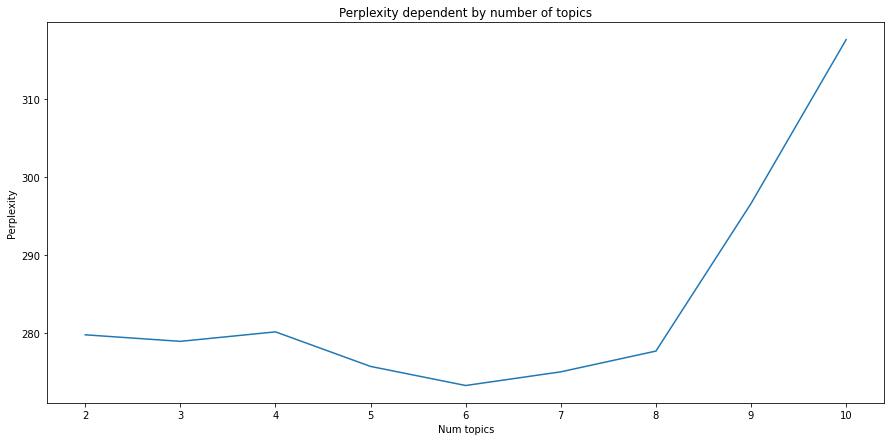
\includegraphics[scale=0.5]{perplexity.png}

Ниже приведены примеры слов, принадлежащие каждой из 6 (с оптимальным значением перплексии) тем:

\begin{tabular}{ | l | l | l | }
\hline
Номер темы & Слова \\ \hline
1 & obama, state, president, government, american, \\ & israel,  policy, country \\ \hline
2 & woman, say, work, health, year, senate, group, \\ & government,  support, company \\ \hline
3 & call, get, work, see, want, know, good, also, think, tomorrow \\ \hline
4 & secretary, office, state, meet, room, department,  \\ &  arrive, route, depart, private \\ \hline 
5 & state, information, benghazi, department, doc, case, subject, \\ & iran, agreement, house \\ \hline
6 & cheryl, gov, fyi, sullivan, state, friday, sunday, branch,  \\ & wednesday, april, january \\ \hline 

\end{tabular}

\newpage

Распределение слов по темам:

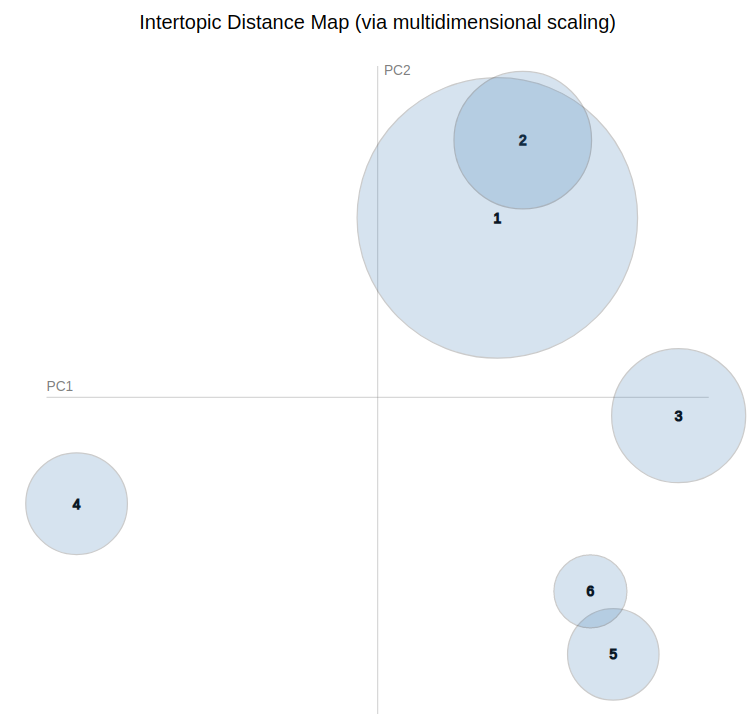
\includegraphics[scale=0.5]{words_map.png}


%\section{Предобработка электронных писем корпорации Enron}

\subsection{Выделение метаданных из сырого текста писем}

Набор данных \textit{Enron} также требует предварительной обработки. К примеру, так выглядит необработная информация одного электронного письма:

\begin{verbatim}
Message-ID: <18782981.1075855378110.JavaMail.evans@thyme>
Date: Mon, 14 May 2001 16:39:00 -0700 (PDT)
From: phillip.allen@enron.com
To: tim.belden@enron.com
Subject: 
Mime-Version: 1.0
Content-Type: text/plain; charset=us-ascii
Content-Transfer-Encoding: 7bit
X-From: Phillip K Allen
X-To: Tim Belden <Tim Belden/Enron@EnronXGate>
X-cc: 
X-bcc: 
X-Folder: \\Phillip_Allen_Jan2002_1\\Allen, Phillip K.\\\'Sent Mail
X-Origin: Allen-P
X-FileName: pallen (Non-Privileged).pst

Here is our forecast
\end{verbatim}

Конечно, анализировать данные (в том числе метаинформацию о письме) в таком формате бессмысленно. Для обработки мы будем использовать библиотеку \textit{email} \cite{bib8}. Данная библиотека позволяет из сырых данных выделить вспомогательную информацию о письме, в частности, библиотека позволяет выделить следующие интересные нам атрибуты:
\begin{itemize}
\item полное содержание письма,
\item дата отправки,
\item адрес получателя,
\item адрес отправителя,
\item тема письма,
\item логин отправителя.
\end{itemize}

\subsection{Выделение содержания писем}

После этого требуется также привести содержание письма в приемлимый для дальнейшего обучения вид. Например, для письма с содержанием ниже мы хотим выделить только единицы, имеющие отношение к сути письма.

\begin{verbatim}

Forwarded by Phillip K Allen/HOU/ECT on 09/12/2000 11:22 AM 

Michael Etringer

09/11/2000 02:32 PM

To: Phillip K Allen/HOU/ECT@ECT
cc:  
Subject: Contact list for mid market

Phillip,
Attached is the list. Have your people fill in the columns 
highlighted in yellow. As best can we will try not to overlap
on accounts. 
Thanks, Mike
\end{verbatim}

Выделение этих единиц происходит в соответствии со следующей последовательности шагов:
\begin{enumerate}
\item Перевод всех символов в нижний регистр.
\item Удаление всех слов, содержащих цифры. Такие слова не несут смысловой нагрузки и, соответственно, влияют на качество обучения в худшую сторону (подавляющее большинство таких слов было получено отправителями по ошибке).
\item Удаление единиц, соответствующих информации о пересланных письмах.
\item Удаление единиц, соответствующих информации о вложениях в письме.
\item Удаление единиц, соответствующих почтовым адресам, присутствующим в тексте писем.
\item Удаление единиц, соответствующих корпоративным именам пользователей.
\item Удаление единиц, соответствующих ссылкам в сети Интернет.
\item Удаление единиц, не несущих смысловой составляющей, в заголовке письма.
\end{enumerate}

Шаги 3-7 выполняются с использованием регулярных выражений. 

В результате, для примера выше, дальнейшая работа будет производиться со следующим текстом:
\begin{verbatim}
contact list for mid market. phillip, attached is the list. 
have your people fill in the columns highlighted in yellow. 
as best can we will try not to overlap on accounts. thanks, mike'
\end{verbatim}


%\section{Нахождение начального треугольника}

Для дальнейшего хода алгоритма требуется найти какой-нибудь начальник треугольник, являющийся валидным или частично валидным. Любой треугольник, который содержит хотя бы вершину, принадлежащую выпуклой оболочке всех вершин исходной сетки, является валидным или частично валидным и подойдет нам как начальный треугольник. На самом деле можно поступить еще проще, если заметить, что среди треугольников, которые касаются $AABB$ исходной сетки, можно найти валидный и соответственно выбрать его в качестве начального.
%\section{Построение \textit{валидной области}}

Для нахождения \textit{валидной области}, мы используем подход, использующий начальный треугольник, найденный ранее.
Также, вместо того, чтобы заранее разбивать все пересекающиеся треугольники, мы будем разбивать только те частично валидные треугольники, которые появлялись в ходе работы дальнейшего алгоритма, чтобы не совершать лишние операции над невалидными треугольниками. Подробнее, алгоритм построения \textit{валидной области} состоит из следующих шагов:

\begin{enumerate}
\item
Каждый треугольник может иметь одно из следующих состояний:
\begin{itemize}
\item непосещенный треугольник,
\item валидный треугольник,
\item частично валидный треугольник.
\end{itemize}
Изначально все треугольники помечаются как непосещенные.

\item
Начальный треугольник, найденный ранее, помечается валидным и добавляется в некоторое множество $\mathbf{S}$.

\item
Если множество $\mathbf{S}$ пусто, перейти к пункту 5. Иначе, достать треугольник $T$ из $\mathbf{S}$.

\item
Для каждого непосещенного треугольника $T_a$, смежного с $T$, если $T_a$ не пересекается с другими треугольниками, он добавляется в $\mathbf{S}$. В противном случае, $T_a$ помечается частично валидным и добавлется в другое множество $\mathbf{P}$. $T_a$ добавляется в $\mathbf{P}$ вместе с информацией о ребре $e_p$, которое являлось смежным для $T$ и $T_a$.

\item
Если множество $\mathbf{P}$ пусто, перейти к пункту 7. Иначе, достать частично валидный треугольник $T_p$ и его ребро $e_p$ из $\mathbf{P}$.

\item
Триангулировать $T_p$ (детали в секции 2.5). Продолжить построение \textit{валидной области} с помощью $T_p$ и его подтреугольников (как описано в секции 2.6). Если другой начальный треугольник найден, он добавляется в $\mathbf{S}$ и нужно перейти к пункту 2. Иначе, перейти к пункту 4.

\item Построение \textit{валидной области} завершено.

\end{enumerate}


%\section{Триангуляция}

Частично валидный треугольник $T_p$ имеет некоторое количество отрезков пересечений с другими треугольниками. Триангуляция на этом шаге выполняется для того, чтобы: (1) разделить $T_p$ на подтреугольники, которые содержат отрезки пересечений в качестве своих сторон, (2) продолжить построение внутри сетки из полученных подтреугольников.

Подробнее, шаги для (1) следующие:

\begin{enumerate}
\item Разделить каждую сторону треугольника $T_p$ всеми отрезками пересечений $\{s_i\}$.
\item Разделить каждый $s_i$ всеми другими отрезками пересечений.
\item Триангулировать $T_p$ с помощью двумерной триангуляции Делоне с ограничениями (\textit{2D constrained Delaunay triangulation}) \cite{triangulation} вместе со сторонами треугольника и отрезками пересечений, полученных в $1$ и $2$.

\end{enumerate}
Для полученных подтреугольников, дальнеший алгоритм построения начинается с ребра $e_p$. Подтреугольник, смежный ребру $e_p$ помечается валидным и становится начальным для процесса построения в подтреугольниках. Затем валидная часть $T_p$ распространяется к соседним подтреугольникаам до тех пор, пока не достигнет ребер, являющихся частью отрезков пересечений, которые играют роль ребер-входов в соседние треугольники $T_c$ для следующего шага, описанного в секции 2.6.



%\section{<<Crossing the river>>}

\begin{figure}[h]
  \label{fig:cross}
  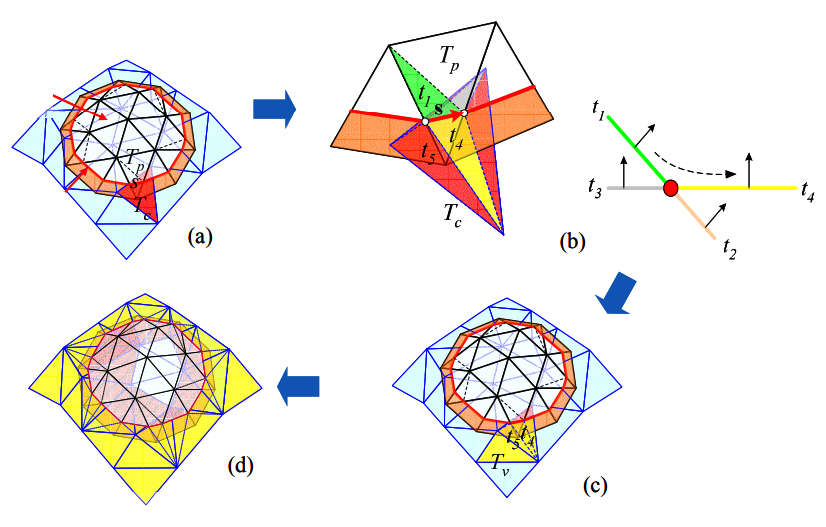
\includegraphics[width=0.7\linewidth]{36.png}
  \centering
  \caption{подробные шаги <<crossing the river>>}
\end{figure}

Процесс построения \textit{валидного региона} может распространиться за самопересечение и переместиться к подтреугольникам соседнего треугольника. Рисунок $2.1$ иллюстрирует подробные шаги распространия внутри подтреугольников частично валидного треугольника. Все начинается с триангуляции соседнего треугольника $T_c$ как в секции 2.5. На рисунке (b) есть два треугольника $t_3$, $t_4$, смежных с ребром-входом. Подтреугольник $t_4$ выбирается как валидный, и будет служить как начальный треугольник в процессе построения внутри подтреугольников $T_c$. В конце концов, как показано на рисунке (c), треугольник $T_v$ будет найден как валидный треугольник и будет добавлен в $\mathbf{S}$.



%\section{<<Сшивание>>}

Так как все частично валидные треугольник были заменены на подтреугольники, а все валидные треугольники уже помечены, в конце нужно оставить только валидные треугольники, а все остальные игнорировать. После этого нужно <<сшить>> ребра самопересечений, определив, что соответствеющие смежные ребра связаны.